\part{Einführung}

\chapter{Aufgabenstellung}
\label{cha:Aufgabenstellung}

\prc{}
\section{Auslöser}

Das ERD (Entity-Relationship-Diagramm) ist seit seiner Entstehung nicht mehr vom Prozess des Datenbank-Designs wegzudenken. Durch dieses Diagramm lässt sich leichter ein konzeptioneller Entwurf für eine Datenbank entwickeln. 
\\

\noindent
Das Erstellen eines solchen Diagramms ist, bis zu einer gewissen Größe des Datenmodells noch per Hand bewältigbar, wird jedoch mit ansteigenden Anzahl von Entitäten schnell komplex und zudem auch mühsam, im Bezug auf die Anordnung der einzelnen Elemente innerhalb des Diagramms.
\\

\noindent
Aus diesem Grund hat Prof. DI Günter Burgstaller das Diplomarbeitsteam beauftragt, ein \textit{englischsprachiges Command-Line-Tool} zu entwickeln, das die Erstellung eines solchen Entity-Relationship-Diagramms vereinfachen soll.
\\

\section{Einsatz und Nutzen}

Bisher ist Erstellung eines ERD mit Applikationen wie dem Oracle SQL Developer Data Modeler eine aufwendige Arbeit. Um zum Beispiel ein Attribut zu einem bestehendem Entity hinzuzufügen sind mehrere Schritte notwendig. Damit dieser Arbeitsaufwand gesenkt wird kommt das Tool zum Einsatz, weil für das hinzufügen eines Attributes lediglich eine Zeile in der Eingabedatei ergänzt werden muss. 
\\

\noindent
Der Nutzen, den man sich von diesem Tool verspricht ist es, sich ein Diagramm in Form von verschiedenen Ausgabeformaten automatisch zeichnen zu lassen, was einem Zeit ersparen soll. Für den Unterricht kann dies bedeuten, dass die Schüler in kürzerer Zeit lernen ein ERD zu lesen und es richtig zu modellieren.
\\

\noindent
Als Eingabe erwartet das Werkzeug eine XML-Datei im XERML-Formatdas von Prof. DI Günter Burgstaller entwickelt wurde.

\chapter{Wieso das ER-Modell?}
\label{cha:Wieso das ER-Modell?}
\prc
\section{Allgemeines zu semantischen Datenmodellen}

Ein Großteil der semantischen Datenmodelle wurde in den 1970er entwickelt \footfullcite{taschenbuch}. Sie dienen der Erstellung einer ersten formalen Beschreibung der Datenbank und werden im Buch ,,\citetitle{taschenbuch}'' wie folgt definiert:

\begin{quote}
	Semantische Datenmodelle beschreiben einen Weltausschnitt als Menge von Gegenständen (Objekten), zwischen denen wohldefinierte Beziehungen existieren und die durch Eigenschaften charakterisiert werden.
\end{quote}

\noindent
Durch die Veranschaulichung von Informationen gehören die semantischen Datenmodelle in der Informationsmodellierung zu den Standards. Das am weitesten verbreitete ist das \textit{Entity-Relationship-Modell} von Peter P. Chen\footnotemark[1]. 

\section{Entity-Relationship-Modell}

\subsection{Grundkonzept}

Im Grunde besteht das ER-Modell aus einer handvoll an Elementen:
\begin{itemize}
	\item Das zu modellierende Objekt genannt Entity und dessen Typ
	\item Die Beziehung oder Relationship und deren Typ
	\item Attribute die die Eigenschaften eines Entitytypen repräsentieren
	\item Attribute die die Eigenschaften einer Beziehung wiedergeben	
\end{itemize}

\noindent
In der Abbildung \ref{Wieso das ER-Modell?} wird eine minimalistischste Version eines ER-Diagramms gezeigt, welches die grafische Darstellung des ER-Modells ist. Das Beispiel selbst gibt den Sachverhalt wieder, dass die Entitytypen ,,wein'' und ,,rebsorte'' über den Beziehungstyp ,,beinhaltet'' miteinander assoziieren.

\begin{figure}[H]
	\begin{center}
		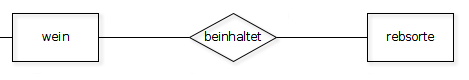
\includegraphics[height=2cm]{images/simplesERD.png}
		\caption{Teil eines simplen ER-Diagramms}
		\label{Wieso das ER-Modell?}
	\end{center}
\end{figure}

\subsubsection{Instanzebene}
\prc
Bei einem \textit{Entity} handelt es sich stets um ein eindeutiges, abgrenzbares Objekt aus der realen Welt oder anders formuliert, um die zu repräsentierende Informationseinheit innerhalb einer Datenbank. In einem ER-Diagramm werden jedoch nicht die einzelnen Entitäten dargestellt, sondern eine Menge von ihnen, die über den \textit{Entitytyp} definiert sind.
\\

\noindent
Zwischen den Entitäten sind Beziehungen definiert, die ebenfalls nicht einzeln, sondern durch den dazugehörigen \textit{Beziehungstyp} in einem Diagramm angezeigt werden.
\\

\noindent
Eine nähere Beschreibung von Entitäten und Beziehungen erfolgt durch die Verwendung von Attributwerten. Jene Werte werden wiederum in Wertemengen zusammengefasst und durch Wertebereiche definiert.
\newline
\noindent
Ein Wertebereich wird im Normalfall durch einen Standard-Datentyp beschrieben. Die gängigsten darunter sind:
\\
\begin{itemize}
	\item \begin{verbatim}
			char
	\end{verbatim} 
	 - für die Darstellung von Zeichenketten
	\item \begin{verbatim}
	integer
	\end{verbatim} 
	 - für ganze Zahlen
	\item \begin{verbatim}
	date
	\end{verbatim} 
	 - für Datumswerte
	\\	
\end{itemize}

\noindent
In der Abbildung \ref{Instanzebene} werden, mit einem Beispiel aus dem Skriptum \citetitle{skriptum}, die Entitäten vom Typ ,,\textit{Abteilung}'' durch die Werte ,,\textit{Verkauf}'' und ,,\textit{Forschung}'' und die Beziehung durch den Wert ,,\textit{leitet}'' dargestellt.
\\

\begin{figure}[H]
	\begin{center}
		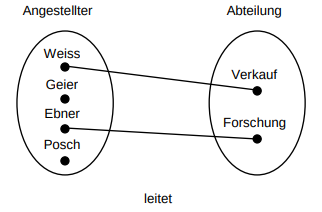
\includegraphics[width=7cm,height=4.5cm]{images/InstanzebeneBsp.png}
		\caption{Beispiel für Instanzebene aus \citetitle{skriptum}
		}
		\label{Instanzebene}
	\end{center}
\end{figure}

\subsubsection{Typebene}

Bei der Typebene geht es um die bereits erwähnten Entity- und Beziehungs-Typen.
\\

\noindent
Unter einem Entitytyp versteht man die Menge der Entitäten mit gleichen Attributen \footfullcite{skriptum}. Diese werden wie in Abbildung \ref{Typebene} durch Rechtecke dargestellt. Ein jeder Entitytyp besitzt einen Namen. Üblicherweise handelt es sich dabei um ein Nomen in der Einzahl.
\\

\noindent
Bei den Beziehungs-Typen kommt das selbe Prinzip zu tragen, wie bei den Entitytypen, nur das es sich beim Namen nicht um ein Nomen sonder meist um ein Verb handelt. Im Skriptum \citetitle{skriptum} wird ein Beziehungstyp so definiert:

\begin{quote}
	Beziehungen, an denen Entities des
	gleichen Entity-Typs beteiligt sind und die dieselbe Bedeutung haben, werden zu einem Beziehungs-Typ
	zusammengefasst. 
\end{quote}

\noindent
Wie bereits in Abbildung \ref{Typebene} ersichtlich, wird ein Beziehungs-Typ durch eine Raute im ER-Diagramm dargestellt.
\\

\noindent
Das letzte grundlegende Element eines ER-Diagramms ist das \textit{Attribut}. Ein Attribut wird durch eine Ellipse dargestellt und ist dem jeweiligem Entity- bzw. Beziehungs-Typen zugeordnet, um dessen Eigenschaften anzugeben. Durch sie wird es möglich, den jeweiligen Typ zu klassifizieren, charakterisieren und identifizieren \footcite{taschenbuch}.

\begin{figure}[!h]
	\begin{center}
		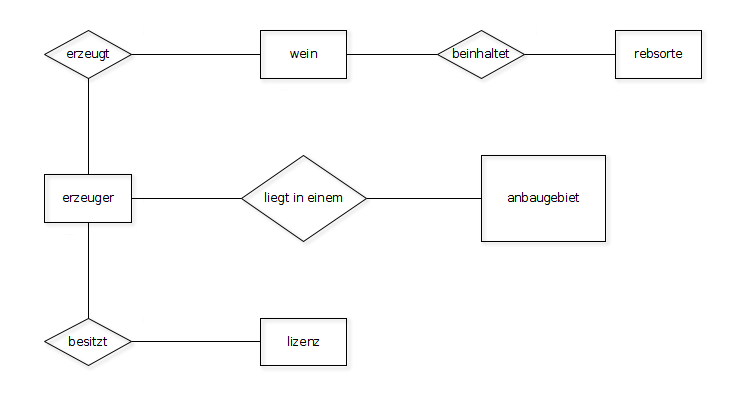
\includegraphics[width=14cm,height=7cm]{images/typebeneBsp.png}
		\caption{Darstellung von Attributen, Entity- und Beziehungs-Typen aus dem Datenmodell Weingut}
		\label{Typebene}
	\end{center}
\end{figure}

\subsection{Beziehungstypen}
\prc
\subsubsection{Kardinalitäten}

Unter der \textit{Kardinalität} eines Beziehungstypen versteht man die quantitative Beschreibung mit Hilfe der (1,M,N)-Notation \footnotemark[3]. Durch dieses Modell erhält man die Information, wie viele Entitäten des einen Entitytypen mit wie vielen Entitäten des anderen Entitytypen in Beziehung stehen können. Dabei wird jede Beziehung in zwei gerichtete Teile aufgeteilt, damit diese getrennt betrachtet werden können.
\\

\noindent
Dem Namen entsprechend kommen bei der Notation als Maximalwerte viele, sprich N bzw. M oder 1 in Frage woraus sich folgende Kombinationen bei den Beziehungstypen ergeben:
\\
\begin{itemize}
	\item 1:1
isting	\item 1:N bzw. N:1
	\item M:N
	\\	
\end{itemize}

\subsubsection{(min,max)-Notation}
\noindent
Bei der (min,max)-Notation handelt es sich um eine Erweiterung der (1,M,N)-Notation, denn durch das Hinzufügen der 0 in den Wertebereich, ist es dem Nutzer möglich ein Minimum für die Beziehungstypen zum Ausdruck zu bringen.
\\

\noindent
Dargestellt werden die Angaben als Intervalle. Außerdem wird bei dieser Notation das ,,N'' in seiner grundlegenden Form durch einen ,,*'' dargestellt \footcite{taschenbuch}. In der nachstehenden Abbildung finden Sie das vorangegangene Beispiel beschrieben durch die (min,max)-Notation.

\begin{figure}[!h]
	\begin{center}
		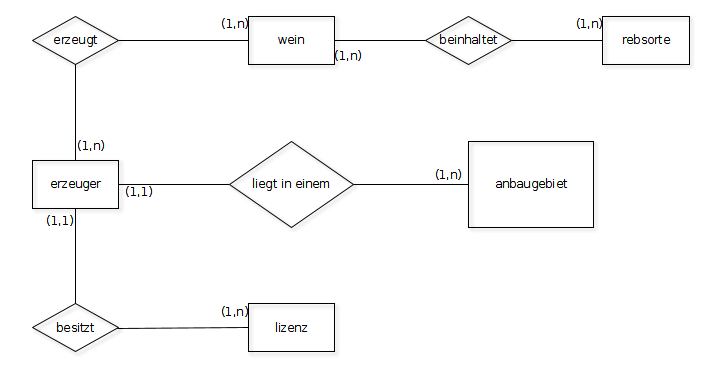
\includegraphics[width=14cm, height=7cm]{images/m_n_notation_bsp.png}
		\caption{ER-Diagramm beschrieben durch (min,max)-Notation}
		\label{MinMaxNotation}
	\end{center}
\end{figure}

\subsection{Attribute}
\prc
Bei manchen Umsetzungen von Datenmodellen kann es zu einem Punkt kommen an dem man die Objekteigenschaft als Attribut oder Entitytyp definieren kann \footcite{skriptum}. Deshalb stellt sich die Frage, wann man eine Informationseinheit im ER-Modell als Attribut oder Entitytyp modelliert. Die folgenden Merkmale helfen bei der Einordnung:
\\

\begin{itemize}
	\item Das Attribut ist immer einem Entitytyp zugeordnet, welcher eigenständig ist.
	\item Der Entitytyp wird durch seine Merkmale definiert. Attribute wiederum durch den erhalten Namen, Wert und Datentyp.
	\\
\end{itemize}

\noindent
Die Attribute werden in zwei Kategorien aufgeteilt. In Schlüssel- und Nichtschlüsselattribute. Ein Schlüssel wird im Buch ,,\citetitle{taschenbuch}'' folgend definiert:

\begin{quote}
	Eine Attributmenge wird als \textbf{Schlüssel} bezeichnet, wenn sie eine eindeutige Identifizierung eines Entities eines Entitytyps ermöglicht und minimal ist.
\end{quote}

\noindent
Der für die Identifizierung verwendete Schlüssel wird \textit{Primärschlüssel (Primary Key)} genannt und üblicherweise unterstrichen um ihn hervorzuheben. Sollte man keinen eindeutigen, minimalen Schlüssel finden wird ein \textit{,,künstlicher'' Schlüssel} verwendet. Diese sind meist Zahlen die pro weiteren Entity um eins erhöht werden.
\\

\noindent
Die bereits erwähnten Nichtschlüsselattribute sind jene, die nicht als Schlüssel geeignet sind und deshalb rein der Charakterisierung dienen \footcite{taschenbuch}. Bei der Zuordnung der Attribute sollte man die Vermeidung von Redundanzen beachten, dass das Merkmal innerhalb des Schemas eindeutig ist und nicht in mehreren Entities, bezüglich auf den Wert des Merkmales, zugeordnet ist.
\\

\section{Andere Vertreter semantischer Datenmodelle}
\prc
Neben dem Entity-Reltionship-Modell von Chen sind während den 70er und 80er Jahren noch weitere semantische Datenmodelle entstanden. Abgesehen vom ,,Relational Model/Tasmania'' von Codd, und dem ,,Functional Data Model'' von Kerschberg \footnotemark[6] gibt es noch das folgende Modell:

\subsubsection{SDM (Semantic Data Model)}

\begin{itemize}
	\item Wurde von Hammer und McLoed 1981 erfunden.
	\item Laut dem Buch \cite{semantischOnlineBuch} befolgt es folgende Grundsätze:
	\begin{quote}
		\begin{enumerate}
			\item To serve as a formal specification mechanism for describing the meaning of a database.
			\item To provide a documentation and interaction medium for database users.
			\item To provide a high-level, semantic based front-end user interface to a database.
			\item To serve as a foundation for supporting effective and structured design of databases.
			\\
		\end{enumerate}
	\end{quote}
\end{itemize}

\subsubsection{UML (Unified Modeling Language)}
\prc
Obwohl der Nutzen von UML hauptsächlich der Modellierung von Software dienen sollte, wurden die Klassendiagramme auch für die Modellierung von semantischen Datenmodellen verwendet.
\\

\noindent
Bei dieser Form der Modellierung werden die Entitytypen als Klassen dargestellt und die Attribute in Form von Klassenattributen. Der Bereich für die Methoden der Klasse bleibt dabei leer. In der Abbildung \ref{uml} sieht man wie laut \cite{sqlDataModeling} die Modellierung eines semantischen Datenmodells aussehen kann.

\begin{figure}[!h]
	\begin{center}
		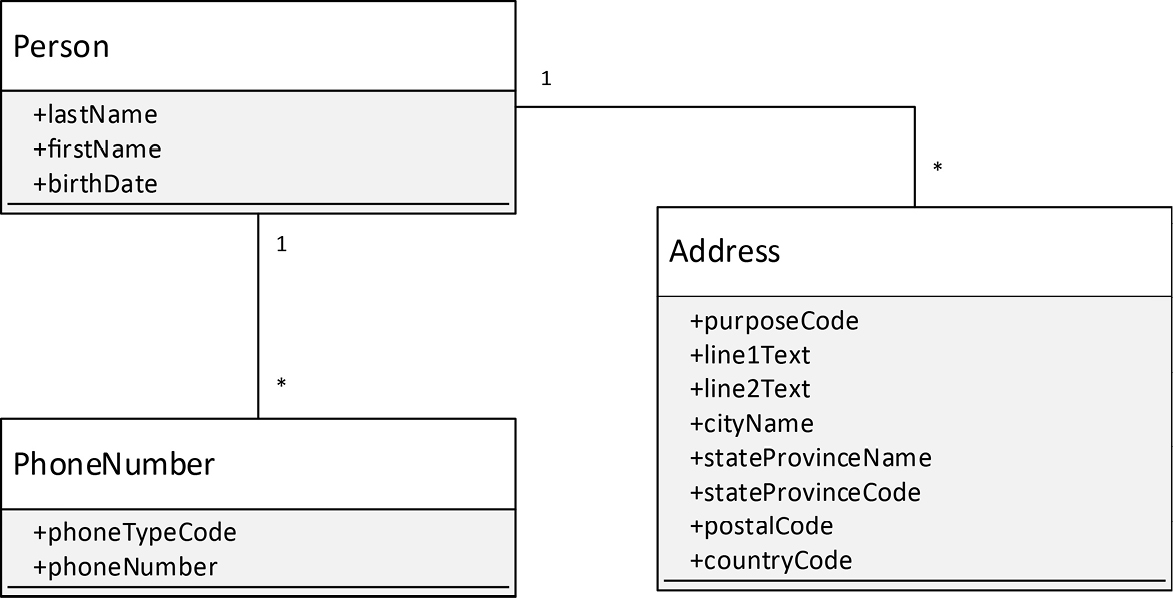
\includegraphics[width=13cm, height=7cm]{images/uml.jpg}
		\caption{Semantisches Datenmodell in UML}
		\label{uml}
	\end{center}
\end{figure}

\noindent
Die Umsetzung mit UML ist aber nicht perfekt und bringt einige Schwachstellen mit sich. Zum einen wäre das die Möglichkeit, dass Attribute durch ein vorstehendes ,,-'' als privat dargestellt werden können. Dieser Umstand ist in der Realität für die Daten einer Datenbank nicht gegeben. Des Weiteren fehlt einem die Möglichkeit Attribute als Schlüssel darzustellen. Dadurch kann ein Datenmodell nicht vollständig über UML realisiert werden \footnotemark[7].


\subsubsection{ORM (Object Role-Modeling)}

Das ORM gehört zu den Fakt-basierten Modellierungen \footcite{sqlDataModeling}. Das besondere an dieser Umsetzung ist die Herangehensweise. Um das Modell am Ende richtig darstellen zu können, hat man als Modellierer Aussagen mit Fakten als Ausgangspunkte. Für das Beispiel in diesem Unterkapitel wurde ein Beispiel aus dem \citetitle{sqlDataModeling} übernommen. Dieses Beispiel hat folgende Aussagen mit Fakten verwendet:
\\
\begin{quote}
\begin{itemize}
	\item Sam Houston works at 123 East Main Street, Dallas, Texas 75208.
	\item Dolly Doolittle works at 123 East Main Street, Dallas, Texas 75208.
	\item Sam Houston lives at 456 Pine Street, Fort Worth, Texas 76104.
	\item Dolly Doolittle lives at 789 Elm Street, Fort Worth, Texas 76104.
	\item Sam Houston’s mobile phone number is 214-555-1212.
	\item Sam Houston’s FAX phone number is 214-555-9999.
	\item Dolly Doolittle’s home phone number is 214-555-1234.
	\\
\end{itemize}
\end{quote}

\noindent
Durch diese Aussagen wird das Diagramm in Abbildung \ref{orm} erstellt. Die abgerundeten Rechtecke repräsentieren hier Objekt der realen Welt oder einen Wert, also eine Zahl oder Zeichenkette. Bei dieser Fakt-basierten Modellierung werden die Attribute durch Beziehungen zu den jeweiligen abgerundeten Rechtecken dargestellt. Das kann man in Abbildung \ref{orm} beim Objekt \textit{Postal Address} sehen \footcite{sqlDataModeling}. 

\begin{figure}[!h]
	\begin{center}
		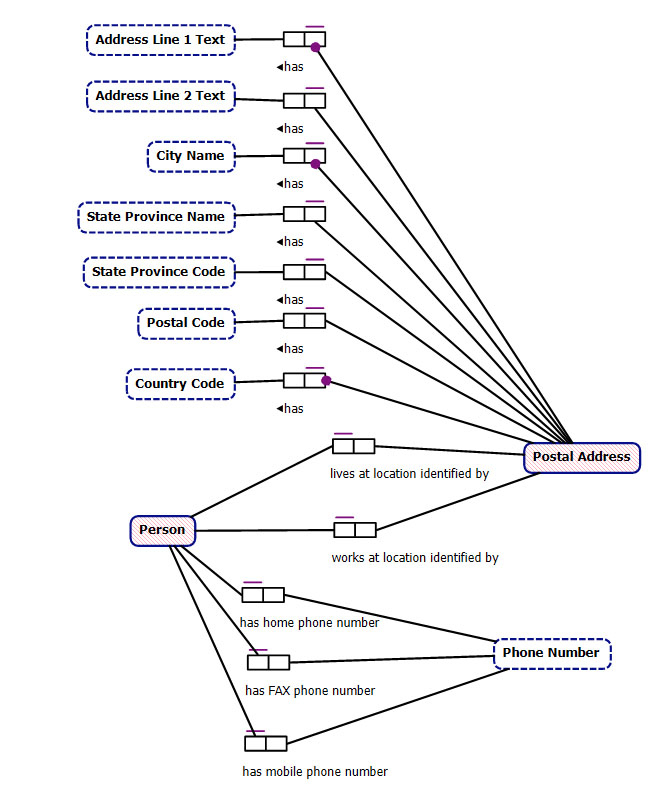
\includegraphics[width=10cm, height=12cm]{images/orm.jpg}
		\caption{Beispiel eines Datenmodells dargestellt in ORM}
		\label{orm}
	\end{center}
\end{figure}